\documentclass[a4paper,12pt]{article}

\usepackage{ifxetex}
\usepackage{amsmath,amssymb}
\ifxetex
	\usepackage{fontspec}
	\usepackage{polyglossia}
\else
	\usepackage{graphicx} % eps support
\fi
\usepackage[margin=20mm]{geometry}
\usepackage[colorlinks=true]{hyperref}
\urlstyle{same}
\usepackage{wrapfig}
\usepackage{subcaption}
\usepackage{authblk}
\usepackage{booktabs}
\usepackage{pstricks}
\usepackage{pstricks-add}

\title{The Study of the Silicon Detector Response for p-Carbon Polarization Measurements at RHIC}

\author[1]{D.~Smirnov\thanks{d.s@plexoos.com}}
\author[2]{D.~Kalinkin}
\author[]{\ldots}

\affil[1]{Brookhaven National Lab}	
\affil[2]{ITEP}

\begin{document}

\maketitle

\begin{abstract}

At the Relativistic Heavy Ion Collider (RHIC) measurements of the proton beam
polarization are carried out by inserting a carbon target in the beam, and
registering the scattered carbon ions with silicon detectors. In this note we
present the results of the analysis of the silicon detector response to carbon
ions and $\alpha$-particles.

\end{abstract}


\section{Motivation}

The RHIC polarimetry is based on the measurement of the recoil from elastic
scattering of the proton beam on a fixed target in the Coulomb nuclear
interference (CNI) energy regime. In this study we focus on the four p-Carbon
polarimeters with ultra thin carbon targets which can be briefly moved into the
beam. In the collider the polarization of each proton beam is measured by two
p-Carbon polarimeters installed in the yellow and blue accelerator rings.

During the 2013 run we observed significant changes in the gain in some of the
silicon detectors. This change of $\lesssim 20~\%$ is worrisome and may cause
significant systematic change in the reported polarization values due to a steep
slope in the $p$-Carbon analysing power within the energy range of interest.


\section{Measurement and Results}

The detectors produced by the BNL instrumentation group have 12 one-millimeter
silicon strips. The detector gain is normally monitored with calibration runs
when there is no beam in the machine. For the calibration purposes we use
$\phantom{A}^{??}$Am and $\phantom{G}^{??}$Gd radioactive sources emitting
$\alpha$-particles with XXX and XXX energies correspondingly.

Starting April XX, 2013 calibration runs were taken automatically after the beam
dump at the end of every RHIC store.


\subsection{Energy calibration with $\alpha$-particles}

The energy of the recoil carbon ions can be reconstructed from either the
amplitude or the integral of the signal in the silicon detector. In order to
convert these values from ADC counts to the energy scale units we need to obtain
properties of our calibration curve i.e. calibrate. One of the possible
calibration procedures is alpha calibration. The idea is to put low intensity
fixed energy alpha source somewhere in acceptance region of the detector and
then look for the corresponding peak in the distribution of particles by ADC
bins. Alpha source energy and position of this peak give us fixed point on the
calibration curve.

At the moment, two polarimeters (Y1D and B1U) has only a single americium source
($E_{\text{Am}} = 5486.0\text{ MeV}$), while other two (Y2U and B2D) has also
additional gadolinium source ($E_{\text{Gd}} = 3271.21\text{ MeV}$). Before now
only americium point was used, the relation between americium energy
$E_{\text{Am}}$ and peak position $\mu_{\text{Am}}$ was called americium gain.
Conversion from ADC counts were performed by multiplying by this value.

Information about gadolinium peak can tell us more about our calibration curve.
For instance we can take gadolinium gain and linear two-point (americium and
gadolinium) fit slope and compare them to americium gain
(Fig.~\ref{fig:gain_relations}).

\begin{figure}[p]
\begin{subfigure}[b]{0.5\textwidth}
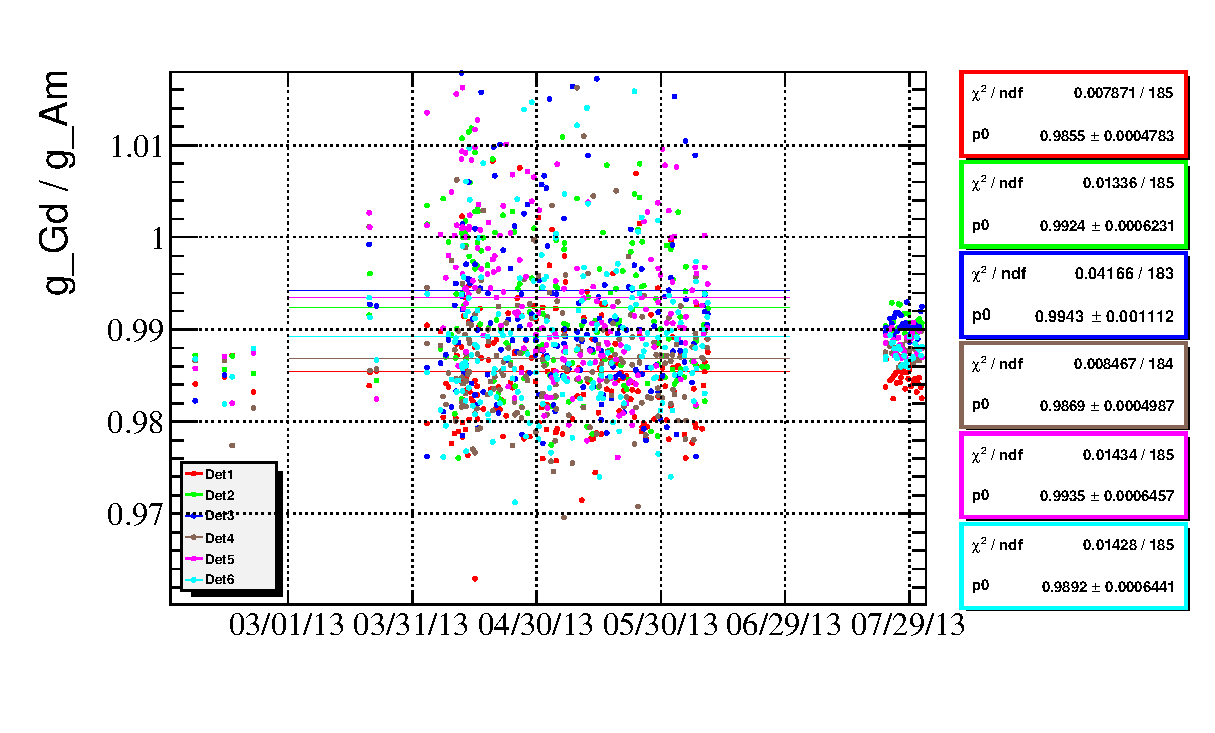
\includegraphics[width=\textwidth]{gfx/run13_alpha_study/Y2U/c_chGdGain_over_AmGain_by_day_Y2U.eps}
\caption{Relation of gadolinium and americium gains}
\end{subfigure}
\begin{subfigure}[b]{0.5\textwidth}
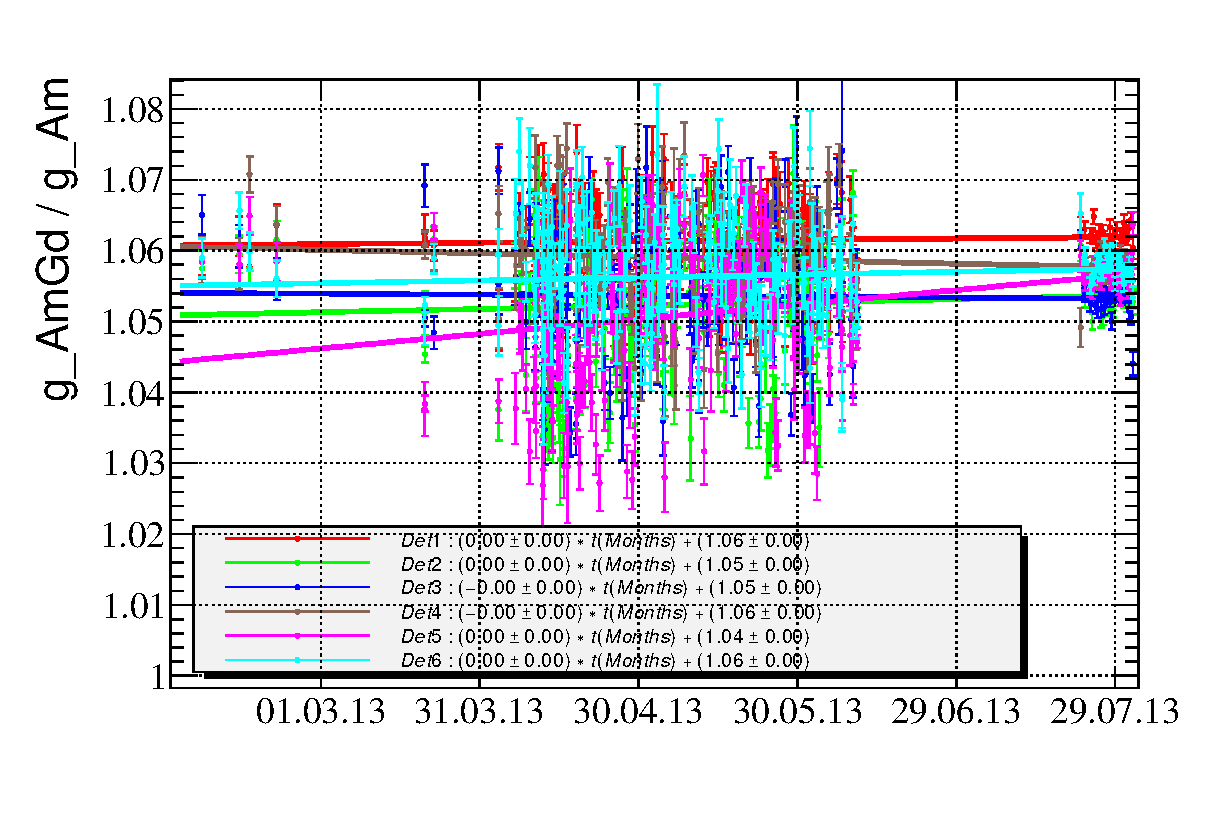
\includegraphics[width=\textwidth]{gfx/run13_alpha_study/Y2U/c_chAmGdGain_over_AmGain_by_day_Y2U.eps}
\caption{Relation of two-point (americium and gadolinium) linear fit slope and americium gain}
\end{subfigure}
\caption{Comparison of different approaches to gain calculation (data for Y2D polarimeter).
Cut to remove outliers was applied to this plot.}
\label{fig:gain_relations}
\end{figure}


\subsection{Linearity of amplifiers}

The signal generated in the detector propagates through several stages of
amplification. The linearity of the downstream amplifiers can be simply checked
by attenuating the signal in a place on the signal path preceding the
amplification, and then compare the reduced final amplitude with the expected
one. The shaper boards have a resistive divider with a multiplexer controlled by
software settings. For normal polarization measurements of sub-MeV carbon ions
the on-board attenuator is set to 1, i.e. no signal attenuation. During regular
alpha measurements the attenuator is set to $1/5$. In this study we check the
other two attenuator settings of $1/10$ and $1/3$. The alpha peaks obtained with
these attenuator settings are shown in Figure~\ref{fig:atten_distrib} and the
mean values corresponding to the gaussian fits are listed in
Table~\ref{table:atten}. Note that with the attenuator setting of $1/3$ the Am
peak ends up in the overflow bin as the events are outside of the detector
dynamic range. The cumulative effect of a possible non-linearity in the
amplified signal is checked by using the trivial relation in which the mean of
the peak is expected to scale with the attenuator settings:

\begin{equation}
\lambda_1/\lambda_2 = \mu_1/ \mu_2.
\label{eq:atten_linearity}
\end{equation}


\begin{table}[htb]
\caption{The mean positions of the Am and Gd alpha peaks at different attenuator settings.}
\centering

\begin{tabular}{clrr}
\toprule
Attenuation $\lambda$ & Alpha Run Id      & Am Mean, ADC      & Gd Mean, ADC \\
\midrule
$\frac{1}{10}$  & \small{atten\_1\_over\_10.yel2.alpha0}  & $77.0\pm0.7$      & $44.2\pm0.4$ \\
\addlinespace
$\frac{1}{5}$   & \small{13\_310713.yel2.alpha0}          & $154.9\pm2.7$     & $88.9\pm1.5$ \\
\addlinespace
$\frac{1}{3}$   & \small{atten\_1\_over\_3.yel2.alpha0}   & ---\hspace{20pt}  & $149.4\pm2.5$ \\
\bottomrule
\end{tabular}

\label{table:atten}
\end{table}

\noindent
This effect relative to one of the attenuator settings is then simply defined as
$\Delta l = \frac{\lambda_1 \mu_2}{\lambda_2 \mu_1} - 1$. For the three pairs
of measurements we calculate very small deviations from the linear
equation~(\ref{eq:atten_linearity}).

\begin{equation}
\frac{154.9}{77.0 \times 2} - 1 = 0.6\%
\qquad
\frac{88.9}{44.0 \times 2} - 1 = 0.6\%
\qquad
\frac{149.4 \times 3}{88.9 \times 5} - 1 = 0.8\%
\end{equation}


\begin{figure}[p]
\begin{subfigure}[b]{0.3\textwidth}
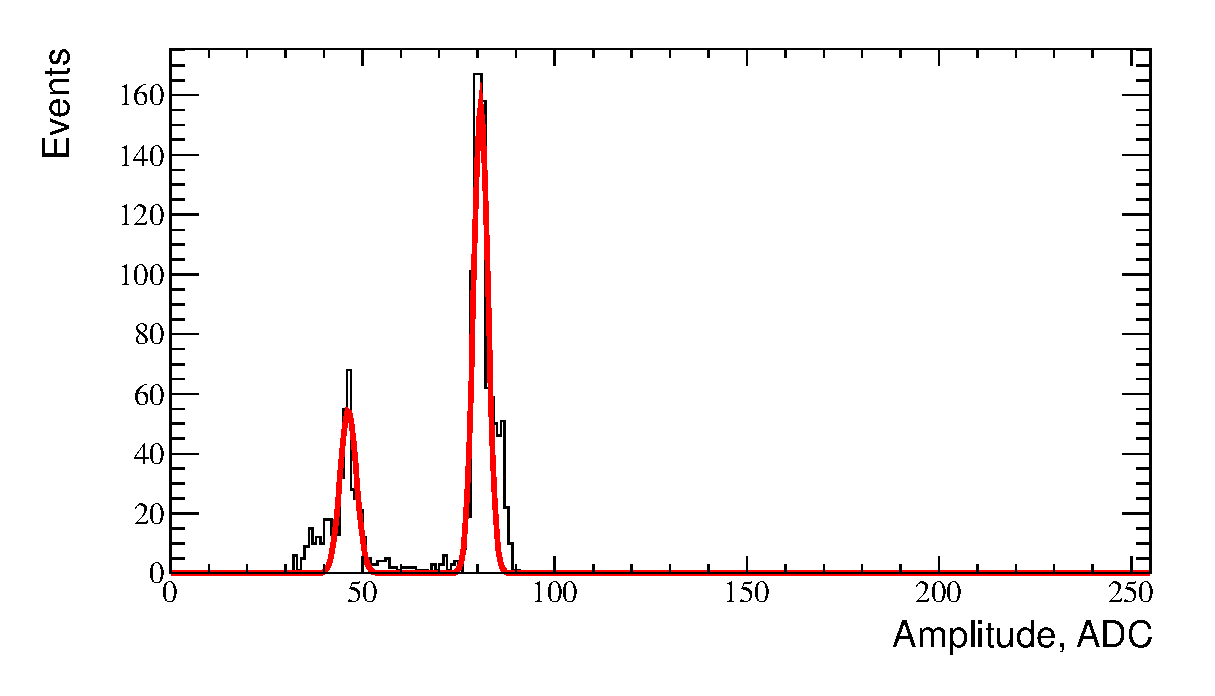
\includegraphics[width=\textwidth]{gfx/atten_1_over_10_ch06.eps}
\caption{$\text{attenuator}=1/10$}
\end{subfigure}
\begin{subfigure}[b]{0.3\textwidth}
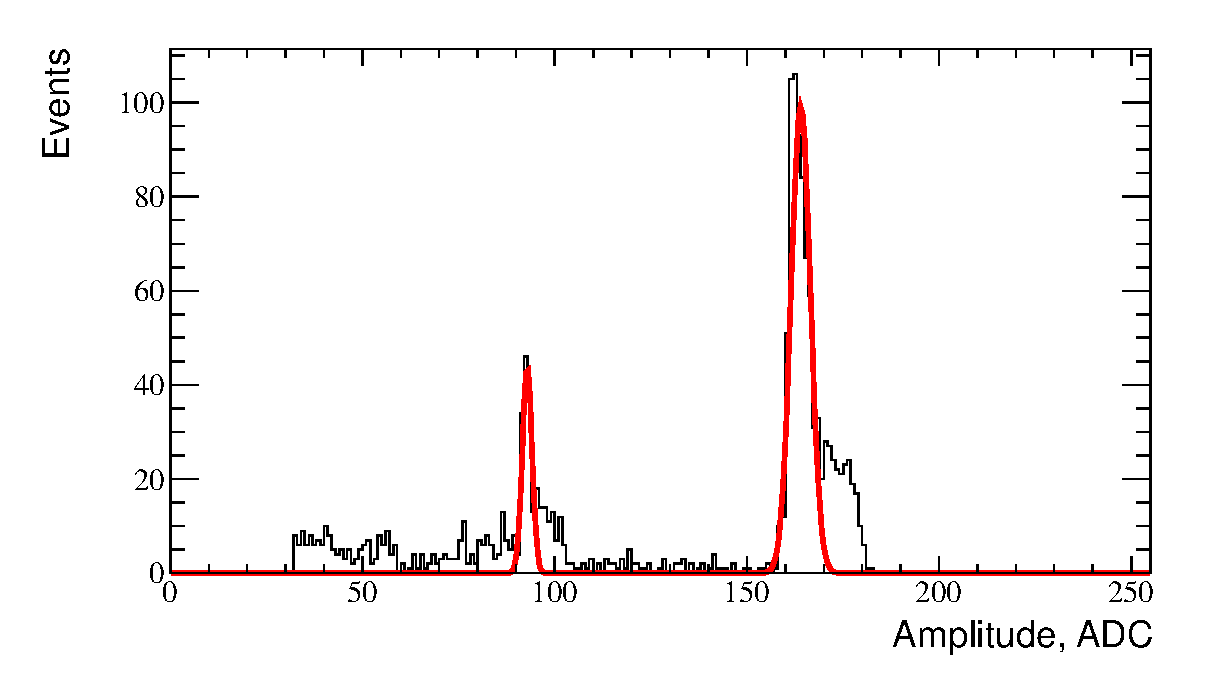
\includegraphics[width=\textwidth]{gfx/atten_1_over_5_ch06.eps}
\caption{$\text{attenuator}=1/5$}
\end{subfigure}
\begin{subfigure}[b]{0.3\textwidth}
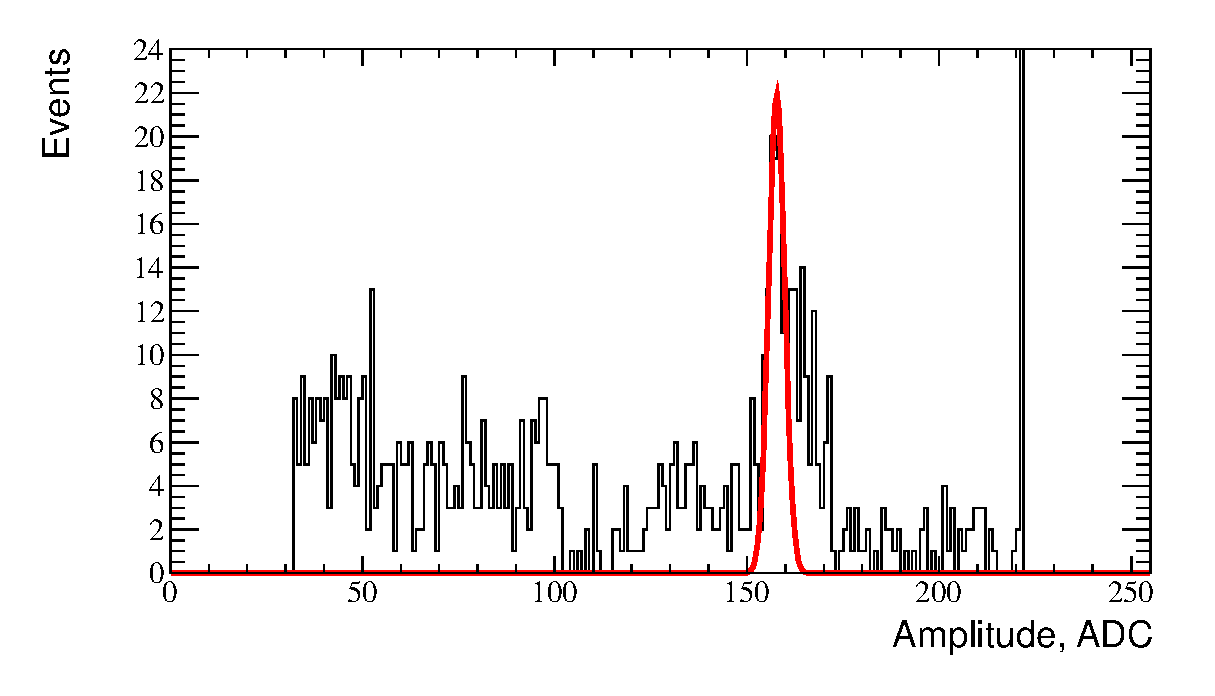
\includegraphics[width=\textwidth]{gfx/atten_1_over_3_ch06.eps}
\caption{$\text{attenuator}=1/3$}
\end{subfigure}
\caption{Alpha peaks seen with different onboard attenuator settings (Y2U)}
\label{fig:atten_distrib}
\end{figure}

\subsection{Dead layer size}

\begin{wrapfigure}{r}{0.3\textwidth}
\vspace{-30pt}
\begin{center}
\setlength{\unitlength}{0.035\textwidth}
\psset{unit=\unitlength}

\begin{pspicture}(0,0)(10,10) % for debugging add [showgrid=true]

% yaxe
\psStartPoint(0.4,0)\psVector(0,10)
\rput[r](0,10){ADC}

% xaxe
\psStartPoint(0,0.4)\psVector(10,0)
\rput[t](10,0){E}

% adc americium tick
\psline(0.2,7)(0.6,7)
\rput[r](0,7){$\mu_\text{Am}$}

% adc gadolinium tick
\psline(0.2,4)(0.6,4)
\rput[r](0,4){$\mu_\text{Gd}$}

\psline(2,0)(8,8)

\psline(2.3,0.2)(2.3,0.6)
\rput[lt](2.3,0){$E_\text{DL}$}

\psline(5,0.2)(5,0.6)
\rput[t](5,0){$E_\text{Gd}$}

\psline(7.2,0.2)(7.2,0.6)
\rput[t](7.2,0){$E_\text{Am}$}

\end{pspicture}

\end{center}
\caption{Linear approximation calibraion curve}
\label{fig:calib_curve}
\end{wrapfigure}

Our model for silicon detector assumes that there is a layer where our detector
has zero response as a calorimeter, i.e. the dead layer. Adding a gadolinium alpha
source to the setup allows us to put one more calibration point on our
calibration curve. Using americium and gadolinium points we can estimate
the thickness of this layer.

The energy where the linear fit intersects the horizontal axis gives us an
estimate for the initial energy of incident alpha particles which would deposit
all of their energy in the dead layer. While this quantity by itself can be used
to monitor the stability of the dead layer over time, we also present the result
in microns. For this we assume that the gain values for both calibration points
are equal and we write:

\begin{equation}
\frac{\mu_{Am}}{E_{Am} - E^\text{DL}_{Am}} = \frac{\mu_{Gd}}{E_{Gd} - E^\text{DL}_{Gd}},
\label{eq:gain_equality}
\end{equation}

\noindent where $\mu_\text{Am}$ and $\mu_\text{Gd}$ are the mean values of the
alpha peaks measured in ADC units, $E_\text{Am}$ and $E_\text{Gd}$ are the
incident energies of $\alpha$-particles, and $E^\text{DL}_{Am}$ and
$E^\text{DL}_{Gd}$ are the energy losses in the dead layer for the respective
alpha sources. The rate at which $\alpha$-particles loose their energy in the
detector changes with the penetration depth. As the dead layer is relatively
thin we can assume that the particles do not loose a significant fraction of
their initial energy and the stopping power is approximately constant over this
range. With a linear approximation for the total losses we have:

\begin{equation}
E^\text{DL}_\text{Am} \simeq x_\text{DL} \lambda_\text{Am} \qquad
E^\text{DL}_\text{Gd} \simeq x_\text{DL} \lambda_\text{Gd}
\label{eq:linear_loss}
\end{equation}

\noindent
with values for the stopping power $\lambda_\text{Am} = $ and $\lambda_\text{Gd}
= $ taken from \cite{ASTAR_database}. Combining (\ref{eq:gain_equality}) and
(\ref{eq:linear_loss}) we obtain the following formula for the size of the dead
layer:

\begin{equation}
x_{DL} = \frac{\mu_{Gd} E_{Am} - \mu_{Am} E_{Gd}}{\mu_{Gd}\lambda_{Am} - \mu_{Am}\lambda_{Gd}}
\label{eq:x_dl}
\end{equation}

The thickness of the dead layer thus extracted from the all available
calibration runs in Run~13 are shown in Figure~\ref{fig:x_dl}. The average size
of the dead layer is estimated to be within 1 to 1.3 $\mu m$.

\begin{figure}[p]
\begin{subfigure}[b]{0.5\textwidth}
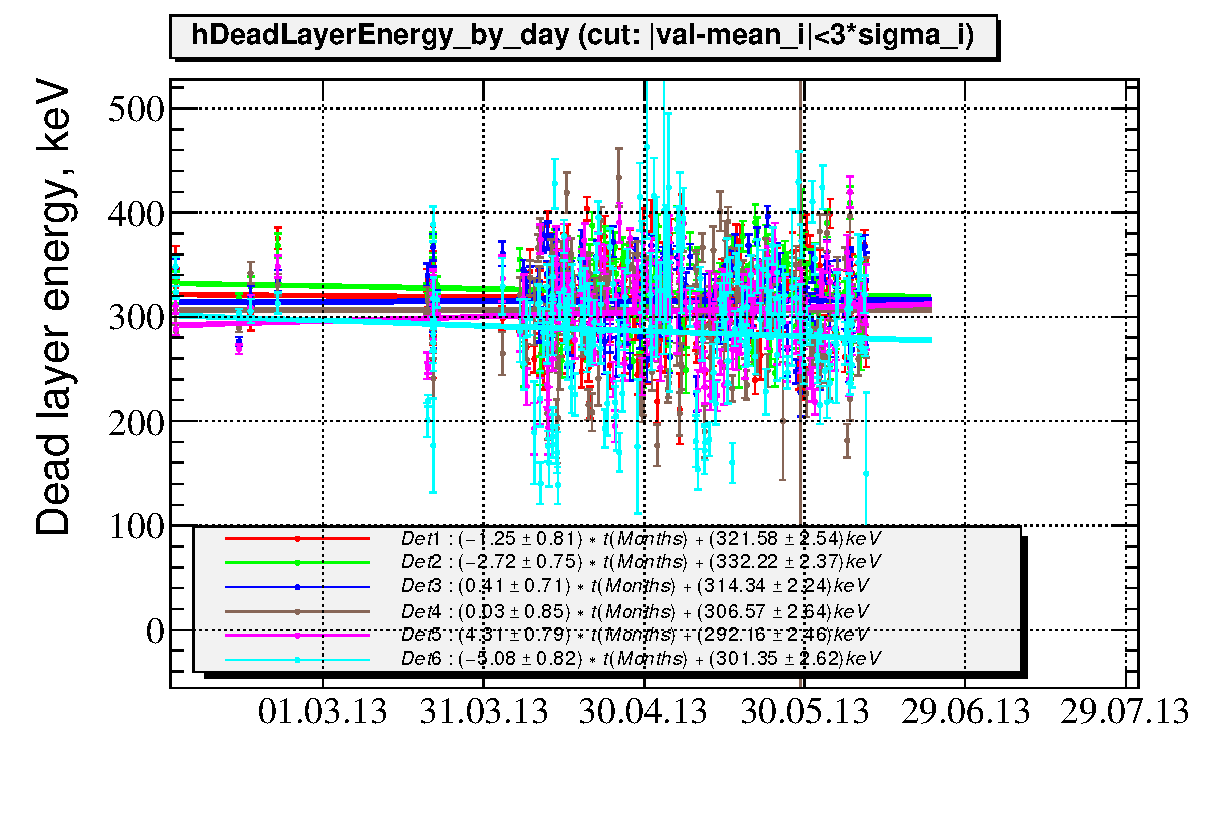
\includegraphics[width=\textwidth]{gfx/run13_alpha_study/B2D/c_chDeadLayerEnergy_by_day_B2D.eps}
\caption{B2D}
\end{subfigure}
%
\begin{subfigure}[b]{0.5\textwidth}
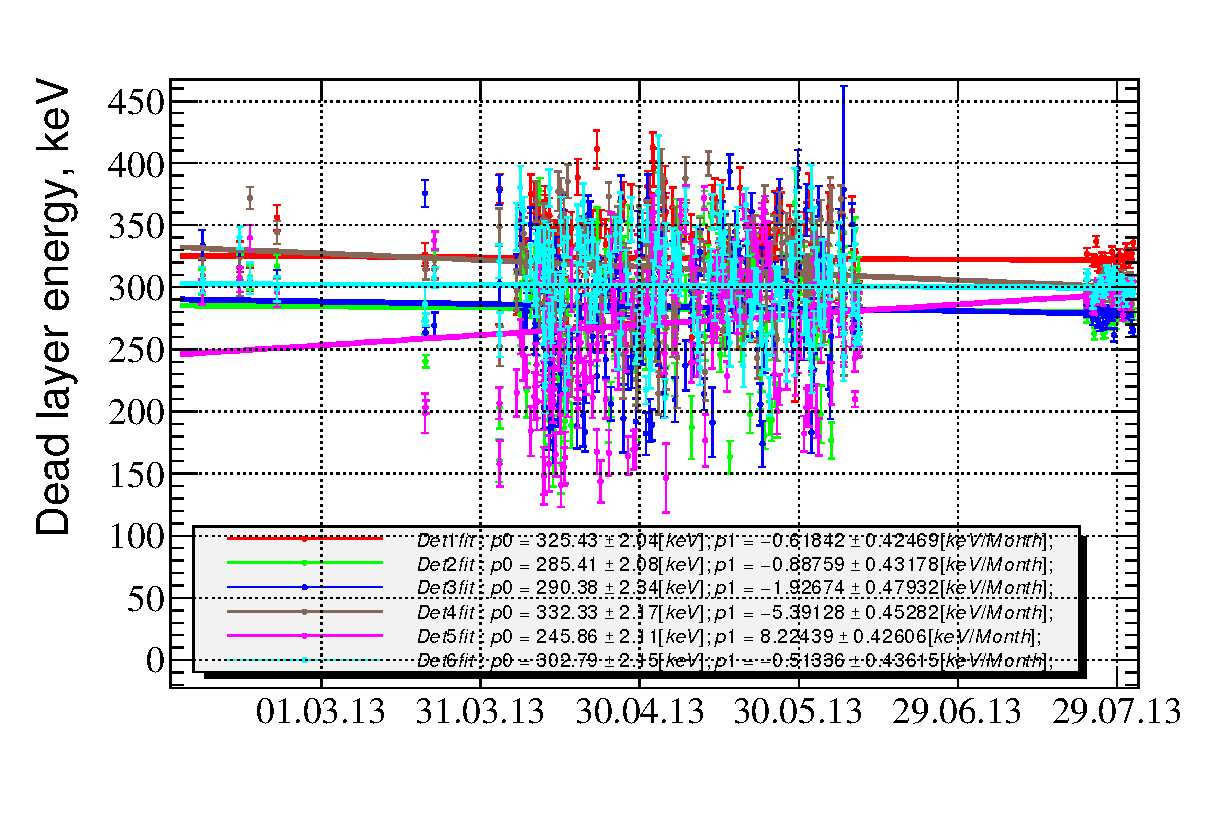
\includegraphics[width=\textwidth]{gfx/run13_alpha_study/Y2U/c_chDeadLayerEnergy_by_day_Y2U.eps}
\caption{Y2U}
\end{subfigure}
%
\caption{$E_{DL}$ (see \ref{fig:calib_curve}) is the missing energy value
extracted from linear fit of the americium and gadolinium points. Cut to remove
outliers was applied to this plot.}
\label{fig:e_dl}
\end{figure}

\begin{figure}[p]
\begin{subfigure}[b]{0.5\textwidth}
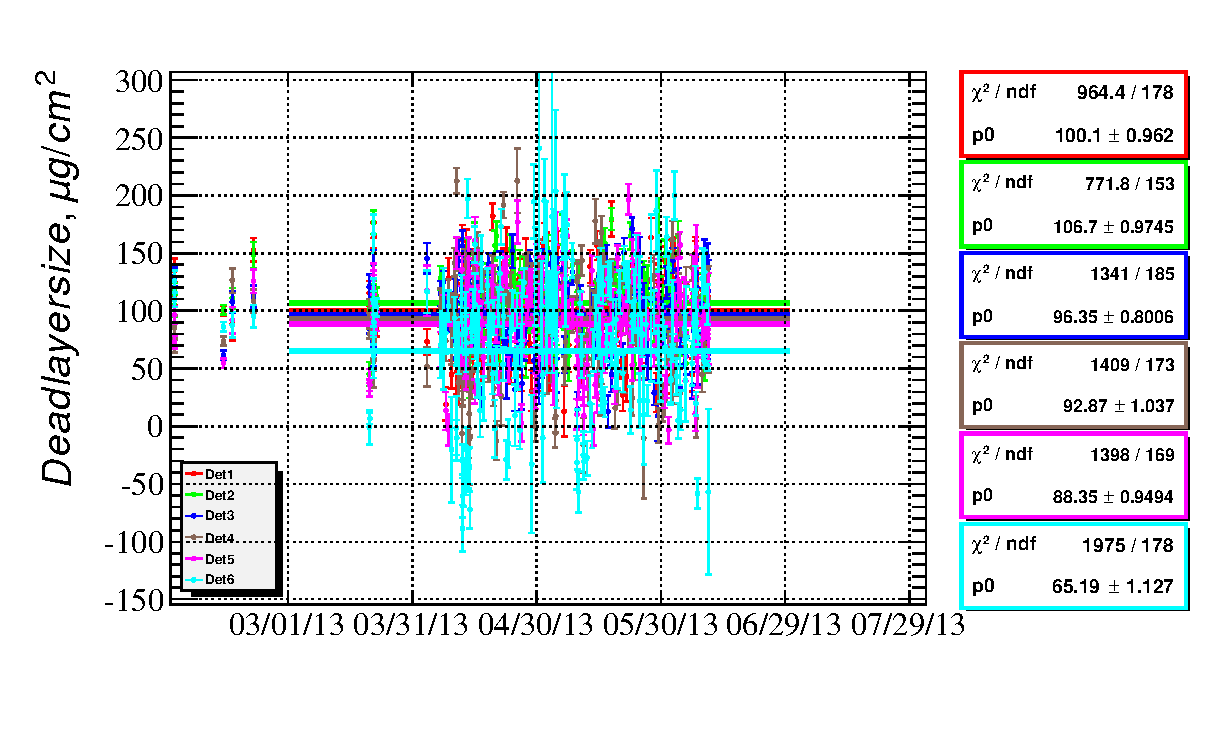
\includegraphics[width=\textwidth]{gfx/run13_alpha_study/B2D/c_chDeadLayerSize_by_day_B2D.eps}
\caption{B2D}
\end{subfigure}
\begin{subfigure}[b]{0.5\textwidth}
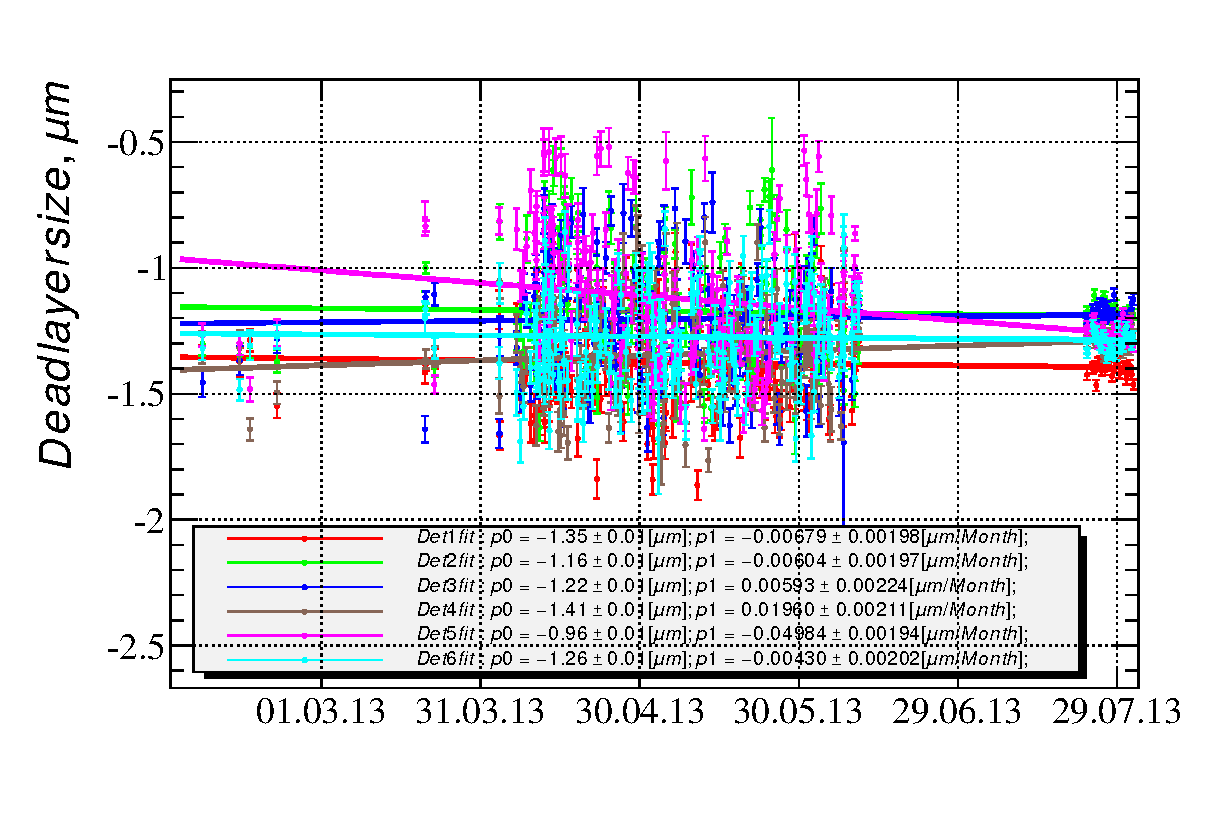
\includegraphics[width=\textwidth]{gfx/run13_alpha_study/Y2U/c_chDeadLayerSize_by_day_Y2U.eps}
\caption{Y2U}
\end{subfigure}
\caption{$x_{DL}$ is the dead layer thickness calculated using formula (\ref{eq:x_dl}). Cut to remove
outliers was applied to this plot.}
\label{fig:x_dl}
\end{figure}

\subsection{Bias current}

% TODO: write something about how out bias current varies over time

On figures~\ref{fig:gain_relations},\ref{fig:e_dl} and \ref{fig:x_dl} there are few measurements
before and after the beam session showing much lower spread. This looks to be a result of some
parameter variation due to beam pickup.

One of the work parameters of our silicon detector that we measure is a bias current -- current
constantly flowing through detector (in this case -- set of 12 strips). Current was measured
for each of the six silicon detectors on all polarimeters, measurements were taken each five
minutes. Values lie mostly in range from $-30$ to $0$~$\mu A$. It was interesting to see how
this current affects calibration characteristics of our detector. For example, it is known 
that higher bias voltage should decrease size of depleted zone, i.e. decrease size of dead layer.
On our plots (Fig.~\ref{fig:bc_vs_xdl}) we see some weak correlation between dead layer size and bias
current.

\begin{figure}[p]
\begin{subfigure}[b]{0.5\textwidth}
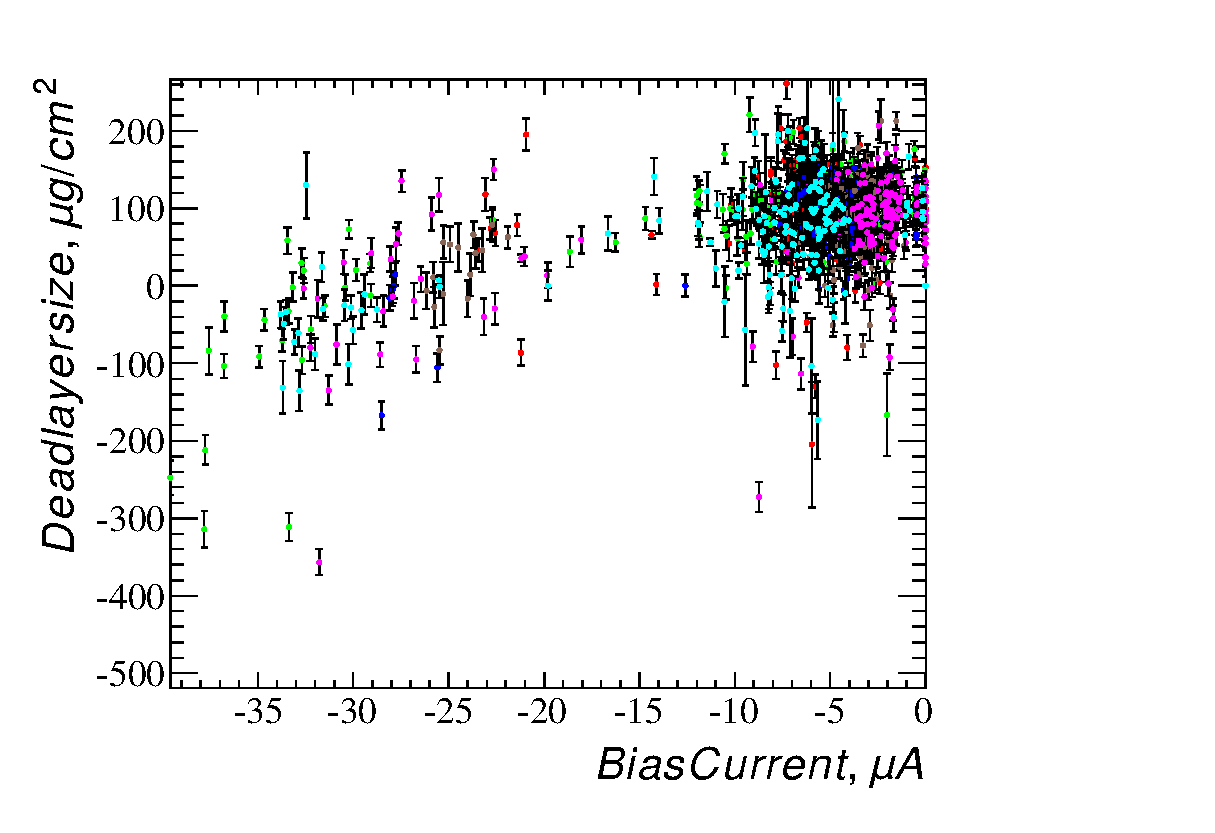
\includegraphics[width=\textwidth]{gfx/run13_alpha_study/B2D/c_hBiasCurrent_DeadLayerSize.eps}
\caption{B2D}
\end{subfigure}
\begin{subfigure}[b]{0.5\textwidth}
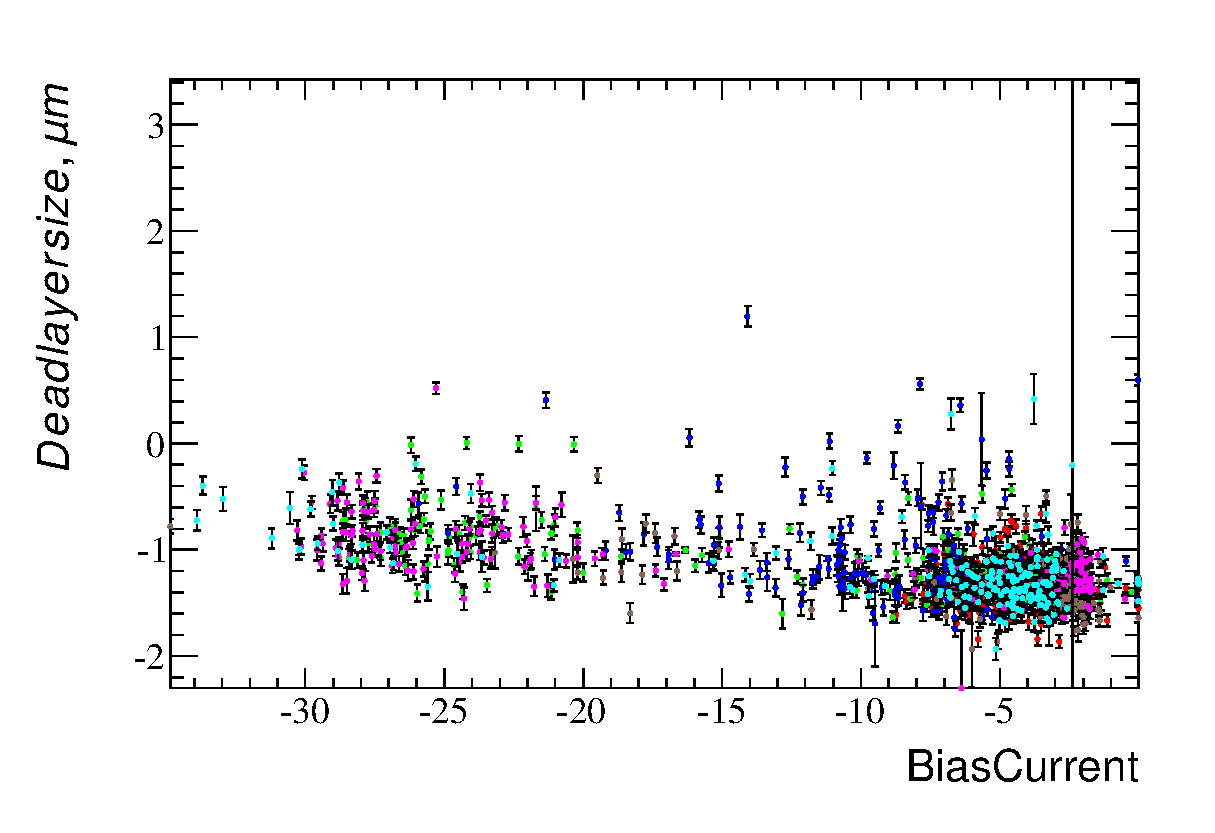
\includegraphics[width=\textwidth]{gfx/run13_alpha_study/Y2U/c_hBiasCurrent_DeadLayerSize.eps}
\caption{Y2U}
\end{subfigure}
\caption{Bias current versus dead layer size dependency}
\label{fig:bc_vs_xdl}
\end{figure}

Much stronger correlation is seen when we compare bias current with gain (Fig.~\ref{fig:bc_vs_gain}).
Bias current during polarization measurement can differ from the bias current in the time of
alpha measurement, so correction to gain value should be applied.

Additional correlation seen on plots \ref{bc_vs_gain-b1u} and \ref{bc_vs_gain-y1d} corresponds to
special set of measurements with varied bias voltage.

\begin{figure}[p]
\begin{subfigure}[b]{0.5\textwidth}
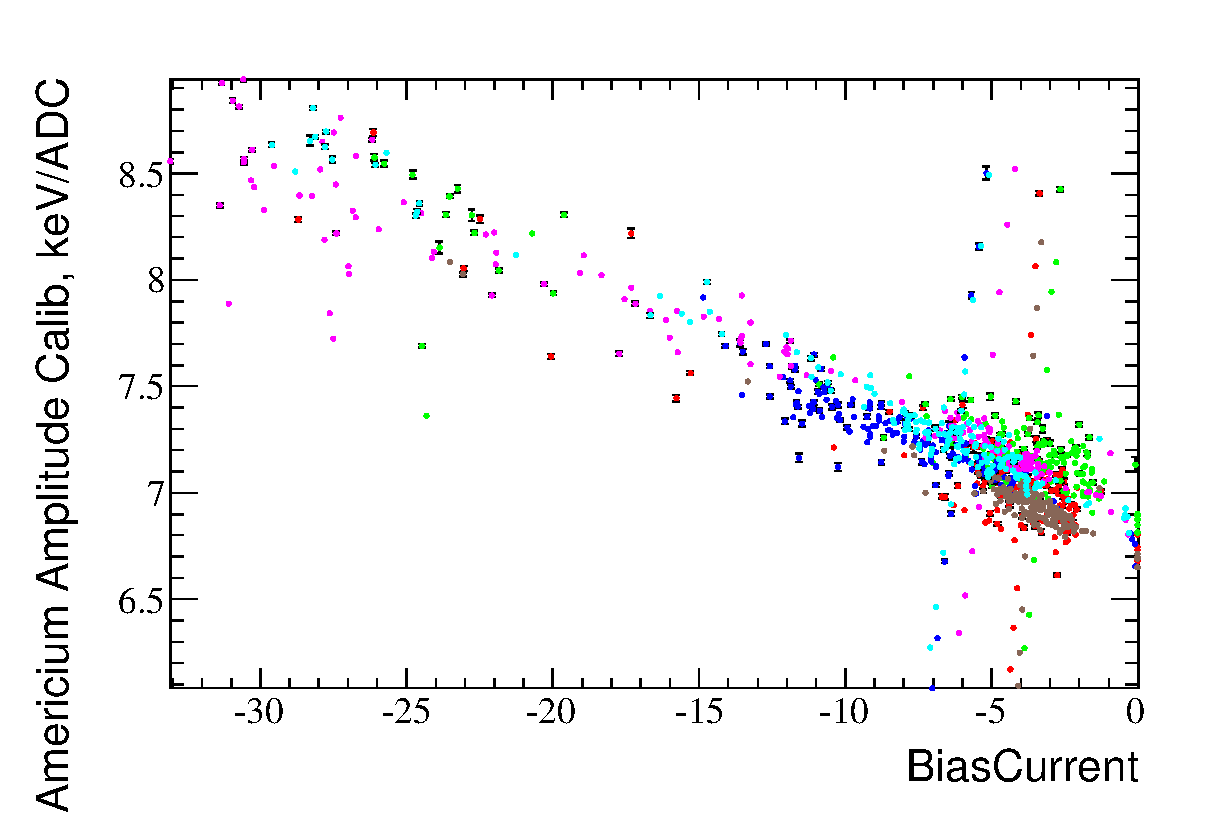
\includegraphics[width=\textwidth]{gfx/run13_alpha_study/B1U/c_hBiasCurrent_AmAmpCoef.eps}
\caption{B1U}\label{bc_vs_gain-b1u}
\end{subfigure}
\begin{subfigure}[b]{0.5\textwidth}
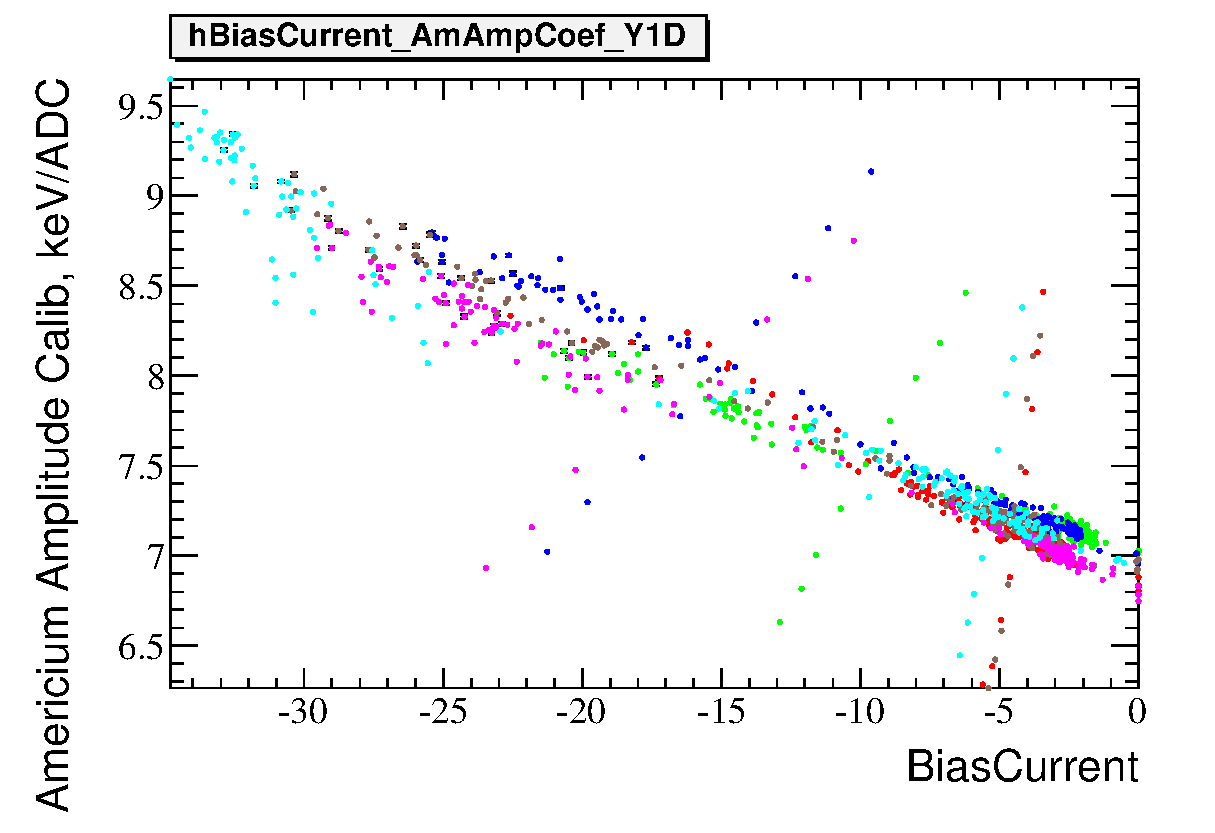
\includegraphics[width=\textwidth]{gfx/run13_alpha_study/Y1D/c_hBiasCurrent_AmAmpCoef.eps}
\caption{Y1D}\label{bc_vs_gain-y1d}
\end{subfigure}

\begin{subfigure}[b]{0.5\textwidth}
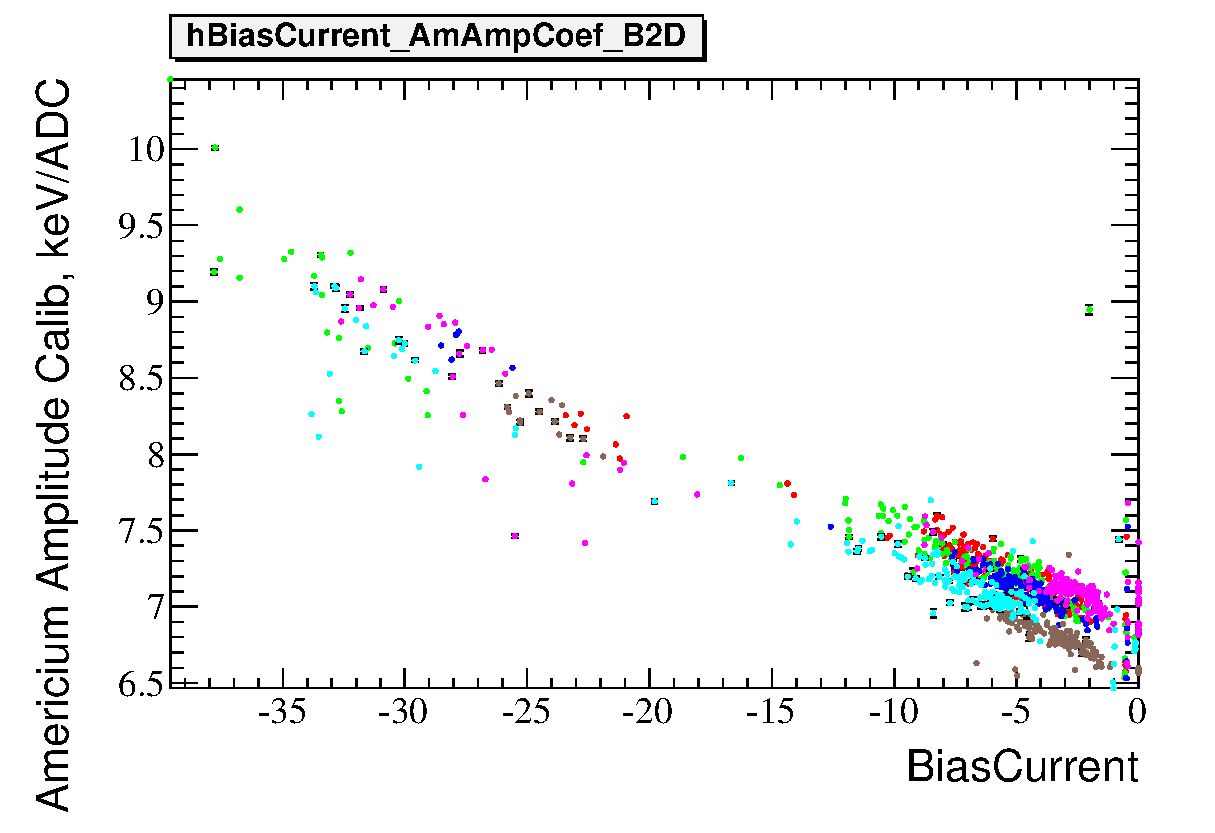
\includegraphics[width=\textwidth]{gfx/run13_alpha_study/B2D/c_hBiasCurrent_AmAmpCoef.eps}
\caption{B2D}\label{bc_vs_gain-b2d}
\end{subfigure}
\begin{subfigure}[b]{0.5\textwidth}
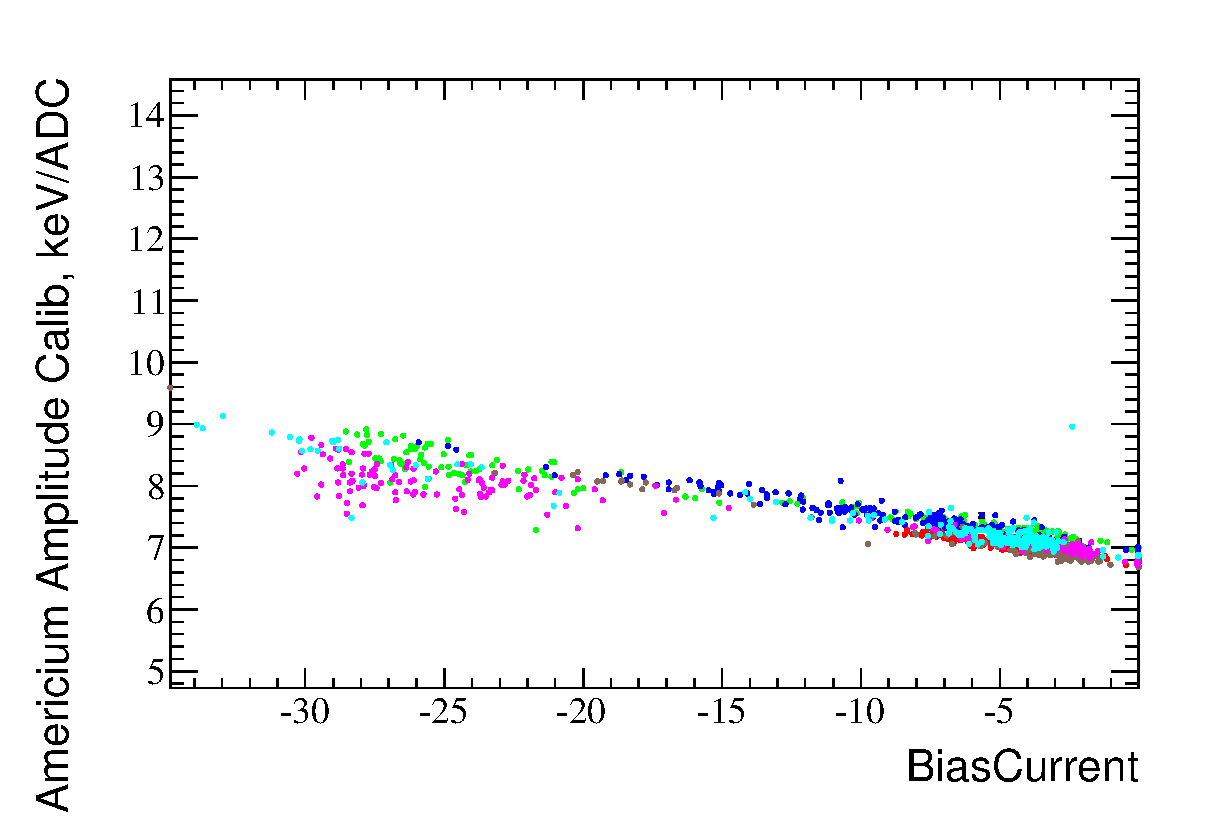
\includegraphics[width=\textwidth]{gfx/run13_alpha_study/Y2U/c_hBiasCurrent_AmAmpCoef.eps}
\caption{Y2U}\label{bc_vs_gain-y2u}
\end{subfigure}

\caption{Bias current versus americium gain ($E_{\text{Am}} / \mu_{\text{Am}}$) dependency}
\label{fig:bc_vs_gain}
\end{figure}

\begin{figure}[p]
\begin{subfigure}[b]{0.5\textwidth}
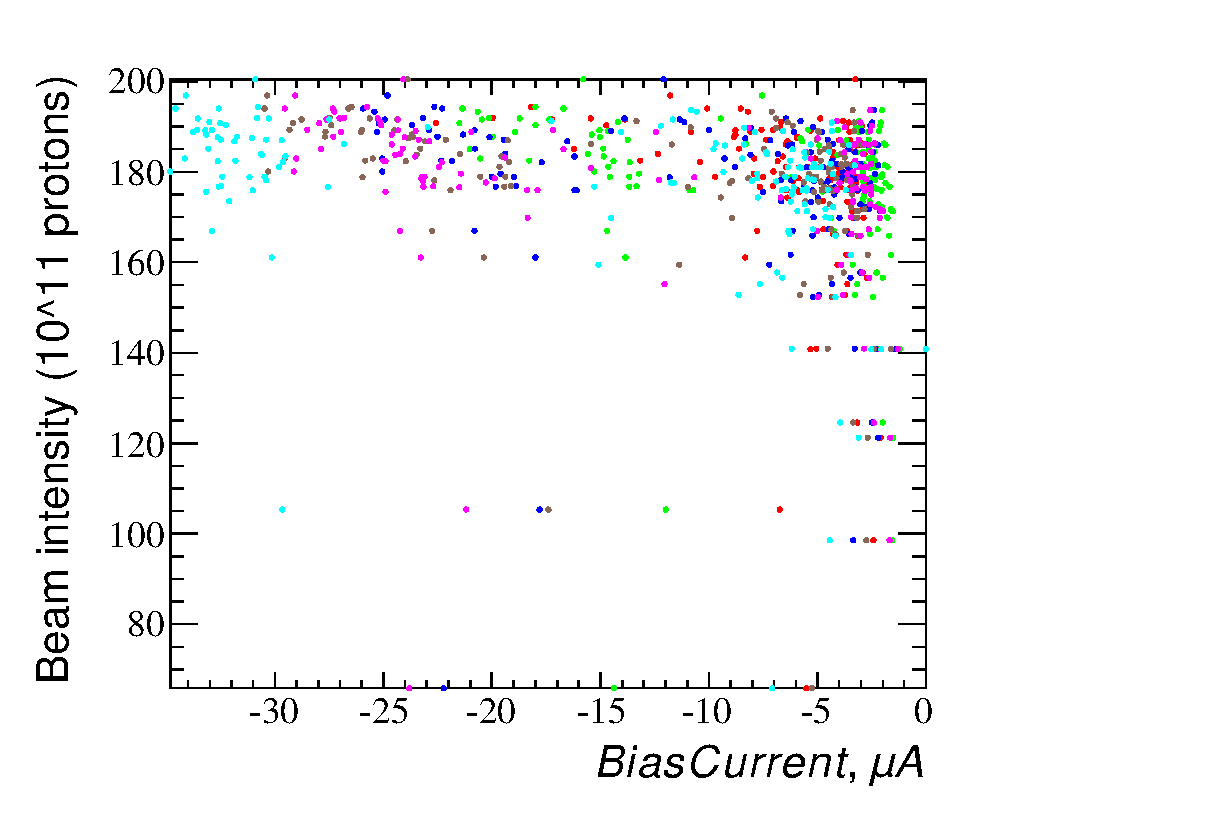
\includegraphics[width=\textwidth]{gfx/run13_alpha_study/Y1D/c_hBiasCurrent_BeamCurrent.eps}
\caption{Y1D}
\end{subfigure}
\begin{subfigure}[b]{0.5\textwidth}
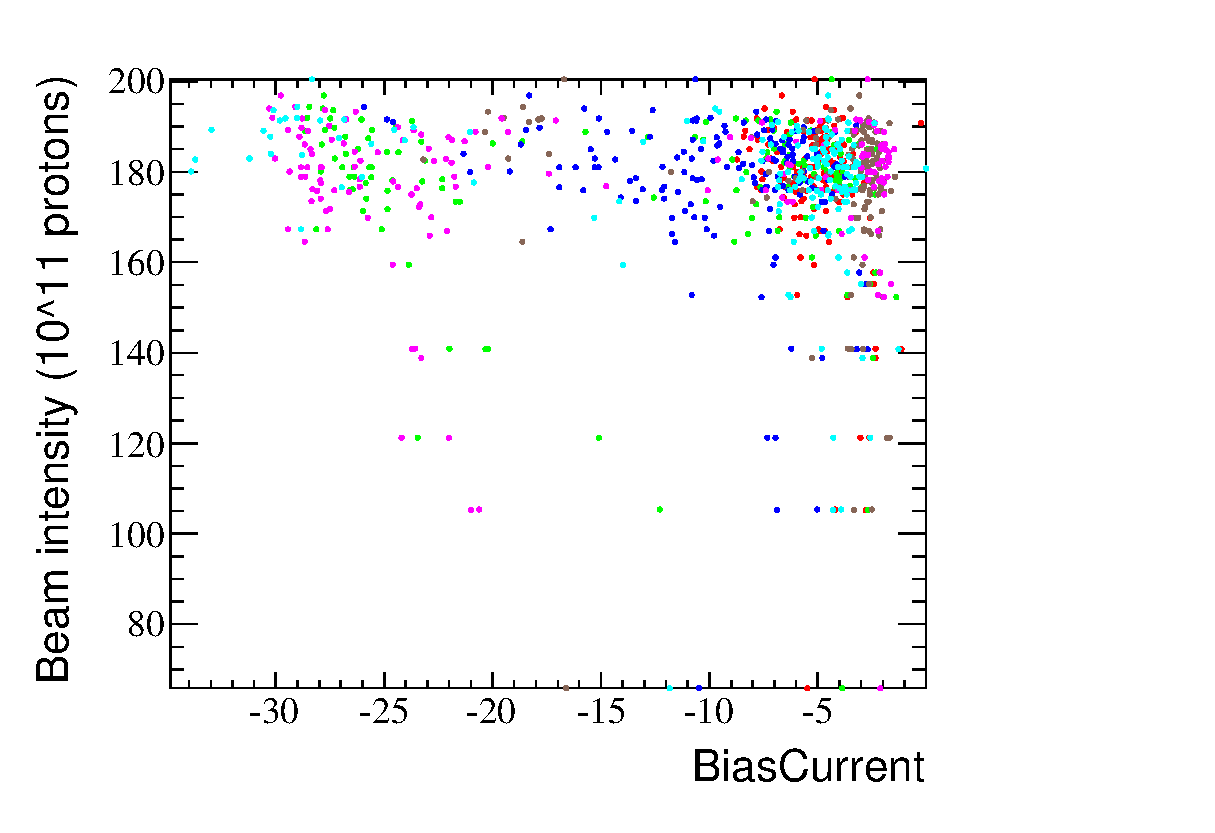
\includegraphics[width=\textwidth]{gfx/run13_alpha_study/Y2U/c_hBiasCurrent_BeamCurrent.eps}
\caption{Y2U}
\end{subfigure}
\caption{Bias current during alpha measurement versus beam current during the fill.}
\end{figure}


\section{Conclusions}

Based on the analysis presented in this note we establish that the changes in
the bias currents in out silicon detectors heavily depend on the beam activity
in the RHIC. At the moment, we do not see that the bias current correlates with
the beam intensity but in further studies we plan to investigate if other beam
or machine parameters have direct impact on the detectors.

We observe a clear correlation between the gain and the bias current.

We do not see a significant radiation damage of the current detectors.

The presence of the two $\alpha$-sources in the polarimeters allowed us to find
a correction for the effective detector gain by taking into account the energy
lost in the dead layer. We find this correction to be at $\approx 5\%$ level
with respect to the nominal calibration procedure with one radioactive source.
In addition, we estimate the thickness of the effective dead layer to be
$\approx 1.1\mu m$. This number significantly disagrees with the value extracted
from the nominal ``banana'' fit to the carbon data where the dead layer is
estimated to be $\approx 0.15\mu m$. A possible explanation for this discrepancy
is that we overestimate the dead layer thickness as measured with
$\alpha$-particles by not taking into account the extra material covering the
source.


\begin{thebibliography}{99} % for less than 10 references use just {9}

\bibitem{astar_database}
ASTAR database. Stopping power and range tables for helium atoms:
\url{http://physics.nist.gov/PhysRefData/Star/Text/ASTAR.html}

\bibitem{cnipol_code}
RHIC polarimetry analysis framework: \url{https://github.com/rhicspin/cnipol}

\bibitem{cnipol_web_rundb}
RHIC polarimetry results: \url{http://www.phy.bnl.gov/cnipol/rundb/}

\end{thebibliography}

\end{document}
